
\documentclass[preprint]{aastex}


\newcommand{\vdag}{(v)^\dagger}
\newcommand{\myemail}{npk@astro.caltech.edu}

%\shorttitle{Design and Construction of the SED Machine}
%\shortauthors{Konidaris, Ben-Ami, \& Quimby}


\begin{document}

\title{The design and construction of the SED Machine}


\author{Nicholas P. Konidaris}
\affil{Caltech}

\author{Sagi Ben-Ami}
\affil{Weizman institute}

\and

\author{Robert Quimby}
\affil{IPMU}


\begin{abstract}
Every year the current group of imaging surveys discovers several thousand candidate supernovae per year. The Spectral Energy Distribution (SED) Machine is a spectrograph designed to classify thousands of transients per year by taking spectra on Palomar's robotic 60-inch telescope. In this paper we present the design and construction of the SED Machine; a spectrograph designed from the bottom up to classify supernovae efficiently on telescopes of apertures up to 3 meter. The SED machine is a ugri imager with a 12x12 minute field and a spectrograph with resolution ($R=\lambda/\Delta\lambda$) 100 covering the wavelength range from 370 nm - 920 nm, fed by a front-end integral-field unit with a 25$\times$25 arcsecond field of view. 
\end{abstract}

\keywords{}
\section{Introduction}

Transient discovery rate is high.

Transient classification rate is low.

Current generation of spectrographs is:
overkill
long-slit, this requires at least one minute per exposure. For a night with twenty targets, this amounts to a 5\% loss in classification efficiency.

The SED Machine is designed to achieve:
science requirements
technical requirements.

\section{SED Machine's Metric}

% Section Status: Start here next, copy edit.

The SED Machine is designed to maximize spectral classifications per unit time. As such, it was designed as a system to:
\begin{enumerate}
\item Operate at the minimum spectral resolution necessary to classify 90\% of supernova over the broadest possible wavelength range.
\item Have a high slit-to-detector efficiency. 
\item Have no mode switching overhead, and few to no moving parts.
\item Require few calibration spectra and images by keeping instrument flexure small (so that few arclamp spectra are needed). 
\item Limit the amount of standard spectra taken by using an atmospheric throughput monitoring camera to measure differential atmospheric absorption.
\item Reduce the amount of time spent acquiring the target with a large field of view integral field unit. Ideally, acquisition is a simple one-shot.
\end{enumerate}

The above scientific requirements flowed down to a number of technical requirements. 

First, based on a number of computer simulations, we decided to adopt a spectral resolution R=$\lambda/\Delta\lambda\sim100$. The details of these simulations are beyond the scope of this paper; however, supernova emission and absorption features are often strong and moving at tens of km s$^{-1}$. 

At this very low spectral resolution $R\sim100$, and given the desire to maximize wavelength coverage and throughput, the team decided to use a prism as the dispersing element. Thus, we could cover over a factor of two in wavelength range without cross dispersion. Furthermore, diffraction gratings have an efficiency functions that is peaked and falls by more than a factor of two at the edge of the order. Prisms, on the other hand, have high and constant throughput. We designed a novel three-element  prism to keep the resolution approximately constant from 370 nm to 920 nm. The spectrograph's low resolution leads to a beam size of 25.0-mm. Thus the instrument is compact and designed to be stiff.

To minimize the number of atmospheric standard spectra taken, we have designed an atmospheric-monitoring camera called the rainbow camera (RC). The term rainbow comes from the simultaneous imaging that takes place over four bands. The partitioning of wavelengths is done with a filter array placed near focus. 

The RC images field stars in four bands around the spectrograph while the spectrograph is integrating. The photometry from the field stars is then compared to that in the Sloan Digital Sky Survey CITEME and AAVSO CITEME and FIXME. The magnitude difference is computed in the SDSS u, g, r, and i bands. Even if the  catalogs do not exist in that part of the sky, the observer can go back on a photometric night and perform their own measurements of the field to back out the extinction. A low-order polynomial is adopted as the correction curve for the spectroscopic observation. Through extensive Monte-Carlo simulations we found that the u-band is the most essential filter for determining atmospheric extinction. Thus, the RC was designed to operate from 320 nm  to 1 $\mu$m.

For the detector, we only considered commercially available fully packaged options. The review consisted of estimating delivered signal-to-noise given read noise, dark current, format size, availability, and cost. We settled on the E2V 42-40 CCD with 13.5 $\mu$m pixels packaged by Princeton Instruments\footnote{We independently measured the quantum efficiency of the Princeton Instruments eXcelon back-illuminated detector. Based on our NIST-traceable photodiode (Thorlabs S120VC s.n.12081057 + PM100USB), we found that the eXcelon QE is about 5\% to 10\% less than advertised; implying it provides little to no improvement over standard and less expensive devices. We also note that we could be wrong. We used a single photodiode (s.n. 12081057) for the measurement, and that the differences between any two photodiodes may be at the 5\% level.} for both the spectrograph and imager. In order to well sample the typical Palomar seeing, we decided on a focal ratio of f/4.9 where typical seeing is sampled with a FWHM of 3.2 pixels. 

The integral-field unit must sample the typical 1.2-arcsecond seeing of the Palomar 60-inch telescope with a pitch of XXXXX. Given the typical pointing of 8 arcsecond RMS a 25-arcsecond full field seemed a comfortable size to ensure that targets usually end up in the IFU. A further advantage of this large field is that is is possible now to simultaneously take spectra of the host galaxy, as well as the transient source.
  
\section{Optical design, construction, and assembly}

The SED Machine's primary purpose is to deliver spectrophotometrically accurate and precise $R\sim100$ spectra of unresolved objects. The SED Machine has an integral field unit with a roughly 30-arcsecond field of view. In order to achieve excellent spectrophotometry the SED Machine uses an imager to monitor the atmospheric throughput. The partition of the focal plane is seen in the raw image shown in Figure~\ref{fig:focal_plane}.

\begin{figure}[h] %  figure placement: here, top, bottom, or page
   \centering
   \includegraphics[width=2.5in]{figures/rc_2013_06_23_01_46_21.pdf} 
   \caption{The SED Machine has a ``rainbow camera'' that takes simultaneous four-band images; and a spectrograph which accesses the field in the 30x30 arc second box. This image was taken at $\alpha$18h47m59 and $\delta$+20:16:37. The large white circle is 9 arcminute in diameter. The plate scale is 0.394"/pixel yield a 13.5 by 13.5 arcminute field of view.  From upper left working clockwise the field is g', u', r', and i'. In a 60-s exposure during full moon the u band sky background is exactly 5.0 times more than the read noise.  }
   \label{fig:focal_plane}
\end{figure}


The focal plane shown in Figure~\ref{fig:focal_plane} shows the g', u', r', and i' filters in a 60-s exposure of a field. A small square shows the outline of the integral-field unit field of view. The spectroscopic field is folded into the spectrograph.

\subsection{IFU and RC: Layout}

The Palomar 60-inch (P60) telescope delivers a focal plan that sits 125-mm behind the mounting plate of the telescope. This back-focus distance forced a number of mechanical design requirements and the instrument is designed around them.

In order to split the spectrograph field, a 5-mm right-angle prism operating in total reflection reflects a 78x78 arcsecond field parallel to the optical breadboard. A 10-mm-diameter expander doublet reimages the telescope focal plane onto a lenslet array through a field lens. The doublet sits on a focus stage that ensures the spectrograph and rainbow-camera are confocal. The lenslet array, through the expander system, is focused on the telescope pupil and delivers pupil images. The system described in this paragraph is known as the front end.

A collimator, prism, and camera follows the front end and focuses the spectra onto a Princeton Instruments PIXIS eXcelon detector. The camera sits on a focus stage that allows spectrograph focus to be adjusted.

The imager is forced to sit behind telescope focus in order to accommodate the spectrograph. Thus the imager has to to reimage the telescope focal plane onto a separate Princeton PIXIS detector. In order to sample the seeing properly, the camera demagnifies the telescope focal plane by about a factor of two. 

The entire optical train is enclosed in a dark black box painted with Avian Black-S (Avian Technologies LLC, New Hampshire, USA). The black paint should deliver total reflectance of less than 3.5\% over the full wavelength range of interest of the SED Machine; however, the paint looks less black than other comparison black materials and it may not have been shaken enough before application.

The discussion of this section describes the optical design, construction, and implementation of the SED Machine. The section is organized by first presenting the integral-field unit (IFU), and second from the rainbow camera. 



\subsection{IFU: Front end}

The heart of the front end of the SED Machine spectrograph is a lenslet array that slices up the field into a grid of telescope images with a pitch of XXX and full field of YYY. A lenslet-based spectrograph described by  disperses these telescope images or micropupils, as if it would disperse a perfect grid of stars.  By adjusting lens pitch and field rotation the lenslet array prescription is responsible for spacing the spectra in the proper way to achieve a large wavelength range and field of view. The classic lenslet spectrograph is TIGER \citep{bacon95} from which most of these concepts are based. An ideal lenslet array will produce an integral field (meaning 100\% fill factor), have little scatter, high throughput, and create a perfect achromatic telescope image.

Another goal of our system is to achieve several-percent spectrophotometry. In order to achieve such accuracy and precision, the flux from spectrum-to-spectrum should not overlap by more than 1\%. The design tension here is to sacrifice field of view in order to minimize spectral overlap. Compared to a variety of instruments that have spectra with five-pixel separation\citep{osiris,p1640,bacon2001,sugai2010}, we chose to sacrifice field of view in order to have 14.5 pixel (14.5 pixel is equivalent to 6 micropupil images) separation. 

\begin{figure}[h] %  figure placement: here, top, bottom, or page
   \centering
   \includegraphics[width=2.5in]{figures/fp.pdf} 
   \caption{This schematic shows the lenslet array's focal plane in units of pixels. The array produces images of diameter $d$ with pitch $p$. An example spectrum is shown as the hatched rectangle. The minimum distance between two spectra is $\epsilon$ with length $L$. Thus the angle the disperser must be tilted relative to the detector is $\theta\sim\arcsin\left(\frac{\epsilon}{p}\right)$.}
   \label{fig:fp}
\end{figure}

Two quantities are fundamental parameters in the design of the SED machine as seen in Figure \ref{fig:fp}. First is the ratio of spot size to pitch $p/d$, and second is the length of the spectrum $L$. The spot size to pitch ratio is defined by the lenslet array and the spectral length is defined by the properties of the spectrograph. At a spectral resolution of $R=100$ and a wavelength range of 370 to 920 nm, it is necessary to have 91 resolution elements (or 219 pixels) per spectrum\footnote{For a constant-resolution spectrograph the number of resolution elements is equal to $N_{res}=\int_{\lambda_a}^{\lambda_b}\frac{R}{\lambda}d\lambda=R\cdot ln\left(\lambda_b/\lambda_a\right)$.}.

With the necessary ratios determined, the next step is to pick the size of the array. The size of the array is a tradeoff between aberrations or scattering. A small lenslet array requires slower optics and thus introduces less geometrical optical aberrations, but at the same time a smaller array has a larger scattering area. 

After laboratory experimentation with several lenslet arrays we found that Advanced Microptical Systems (AMuS) in Germany could produce an array with a roughly 2 to 3 micrometer scattering width between pitches. Compared to some competitors, AMuS' lenslet is made of high UV transparent fused silica and has a high-quality AR coating to ensure excellent throughput. The amount of light scattering for these arrays is the ratio of the area of the scattering region (width $\times$ the perimeter length) to the area of the lenselt. The scattering area is proportional to the ${\rm width/length}$ that for a roughly 0.5-mm pitch lenser with 2-3 $\mu m$ scattering width the several-percent level. Note that for a given pitch, square arrays require a prescription that is roughly 20\% faster than a corresponding hexagon.  In other words, the square lenslets have four long ears of poor image quality whereas hexagons have six much shorter ears. The SED Machine's lenslet array is thus arranged in a set of hexagons.

A CaF2/PBL6Y doublet is used to reimage the small 2x2 mm field delivered by P60 onto the large 25x25 mm lenslet array. The doublet has a field lens that delivers a telecentric beam onto the lenslet array. The telecentric beam is required to ensure that there is no crosstalk between lenslets. The lenslet array 

\subsection{IFU: Collimator and camera}
The primary considerations for the camera is the focal length required to achieve $R\sim100$ spectral resolution. The e2v ccd 42-40 chip employed by SED machine uses pixels that are $13.5\ \mu$ on a side. The $d\theta/d\lambda$ generated by the dispersing prism is such that to achieve $R\sim100$ the camera must have a focal length of 125 mm. In order to magnify the spot diameter (diameter is indicated with the symbol $\diameter$) from the lenslet array to the proper size (24.6 $\mu$ to 32.4 $\mu$) the collimator should operate with a focal length of 95 mm. In that way:
\begin{equation}
{\rm \diameter\ 24.6}\ \mu m\times Magnificaiton = 24.6\mu m\times\frac{f_{camera}}{f_{collimator}}=2.4\,pixel=\diameter32.4\,\mu
\end{equation}


\begin{table}[h]
\caption{SED Machine IFU Focal Lengths and Operating $f/\#$ summary.}
\begin{center}
\begin{tabular}{cccc}
\hline \hline
Tel/Foreoptics & $1.40\times10^5$ mm & $f/8.75$ & Output telecentric \\
Lenslet Array & 2.26 mm & $f/4.5$ & Input/output Telecentric \\
\hline
Collimator & 95.0 mm & $f/4.5$ & Input telecentric\\
\hline
Camera & 125.0 mm & $f/5.9$ \\
\end{tabular}
\end{center}
\label{tbl:focal_lengths}
\end{table}

Based on the arguments above the collimator requires a 95-mm focal length at $f/4$ producing a \diameter24 mm pupil and has a 27-mm (16$^\circ$) full field of view. The collimator is a critical optical component and its design is constrained in five ways. First the collimator must accept a telecentric pupil from the lenslet array. Second the collimator is fed an optically flat field from the lenslet array. Third the collimator and camera cannot induce lateral color or the spectral format will overlap. Fourth the glasses are limited to materials that transmit well in the blue (Calcium Fluoride, Fused Silica, and blue-transmissive glasses). Fifth the collimator must have at least 65-mm of pupil relief in order to put a pupil in the prism and minimize the size of the (expensive) prism.

A collimator and camera were designed by NPK that achieve more than 80\% ensquared energies in a two-pixel box across 90\% of the field. The collimator and camera designs use $i$-line glasses from Ohara in Japan, calcium fluoride from ISP Optical in Rochester United States of America (USA), and spectrosil from Heraeus in Germany. Most elements were polished by Harold Johnson Optical Laboratories in California USA, while calcium-fluoride elements were polished and coated at ISP Optical. Glass and fused-silica elements were coated at Cascade Optical in California USA.

The camera sits on a pair of linear flexure bearings from Riverhawk corporation that is pushed into position by a Newport actuator. The flexures are preloaded by a pair of spring plungers that deliver a preload equal to several-times the weight of the camera. Image quality of the camera is dictated by the temperature of the optical system. To ensure pixel-limited performance the focus stage is required to move on the order of 300 microns, the built focus stage has over 800 microns of free motion.

\subsection{IFU: Prism}

Most modern optical spectrographs use diffraction gratings for their main dispersing element. The SED Machine uses instead a prism which has higher throughput for the low spectral resolution of $\lambda/\Delta\Lambda=100$and allows wavelength coverage over more than a factor of two in wavelength ($370<\lambda\ \left[nm\right]<920$). There are three disadvantage to using a prism: their angular dispersion power is lower than that of a diffraction grating, they have significantly more dispersion in the blue due to the nature of dispersion in optical glass and crystals.


\begin{figure}[h] %  figure placement: here, top, bottom, or page
   \centering
   \includegraphics[width=2.5in]{figures/run_50n.pdf} 
   \caption{A cross-section of the constant-resolution prism. The constant resolution prism has a set of input angles from 34.5 to 51.9 degrees through a PBM2Y/BSL7Y/CaF2 prism. The optical dispersion of the prism is produced by the BSL7Y with the two flanking prisms primarily }
   \label{fig:focal_plane}
\end{figure}



A prism converts some wavelength $\delta \lambda$ into an angle $\delta \theta$. The spectral resolution of the prism is proportional to $\delta n/\delta \lambda$ such that the final spatial separation of two spots separated by two wavelengths $\delta \lambda$ is equivalent to the change in index of refraction $\delta n-1$  times the camera focal length $f_{camera}$. Thus the design of the a prism where $\delta n/\delta \lambda$ holds a constant value was undertaken. A series of approaches was used including looking for closed-form solutions, but in the end the most useful approach was downloading the glass  catalog from Ohara and writing a code that looped over all glass combinations with a metric of keeping $\delta n/\delta \lambda$ constant over a broad range of wavelengths. Afterwards, the list was sorted on the metric and best combination selected. After some experimentation we deemed that a triple prism where the dispersion power is driven by BSL7Y, with two negative flanking prisms of PBM2Y and calcium fluoride. 

As the temperature of the prism changes, the effective index of refraction at a given wavelength changes, and the format of the spectrum swings back-and-forth in the dispersion direction across the focal plane. Temperature changes and {\em time-derivative temperature changes} both affect the resolution and placement of spectra. The formal expression of the amount of change is equal to the angular change as a funcfocal length of the camera

\begin{equation}
\frac{\delta pix}{\Delta T} \propto \frac{f_{camera}}{\rm pixel \ scale}\cdot \frac{\delta \theta}{\delta \lambda} \cdot \frac{\delta \lambda}{\delta n} \cdot \frac{\delta n}{\Delta T}
\end{equation}

where the differential quantities are determined from the glass specification sheets and the optical prescription (i.e., a collimated beam normal to a parallel plate will not exhibit any $\delta \theta$). The variation of temperature with time is parameterized as $\Delta T$. The focal length of the camera and pixel scale are set by the camera prescription and CCD respectively. For this prescription the ratio is roughly 9300 (125-mm camera and 0.0135-mm pixels). The $i$-line glasses have a $\delta n/\Delta T$ of roughly $4\times10^{-6}$; whereas,  $CaF_2$ has a larger and negative value of $\sim-10\times10^{-6}$.

A prism tolerance study on surface quality and material inhomogeneity was performed to ensure that collimated light passing through a prism will yield high quality images. Jenoptix in Florida (formerly Coastal Optical) built a high-quality prism with all faces better than 0.65 fringe in radius and 0.44 fringe in irregularity with all dimensions hit to a fraction of the requested tolerances. The surface irregularity of the delivered prisms increases spot sizes by less than 0.03 pixels in the worst case.


\begin{figure}[h] %  figure placement: here, top, bottom, or page
   \centering
   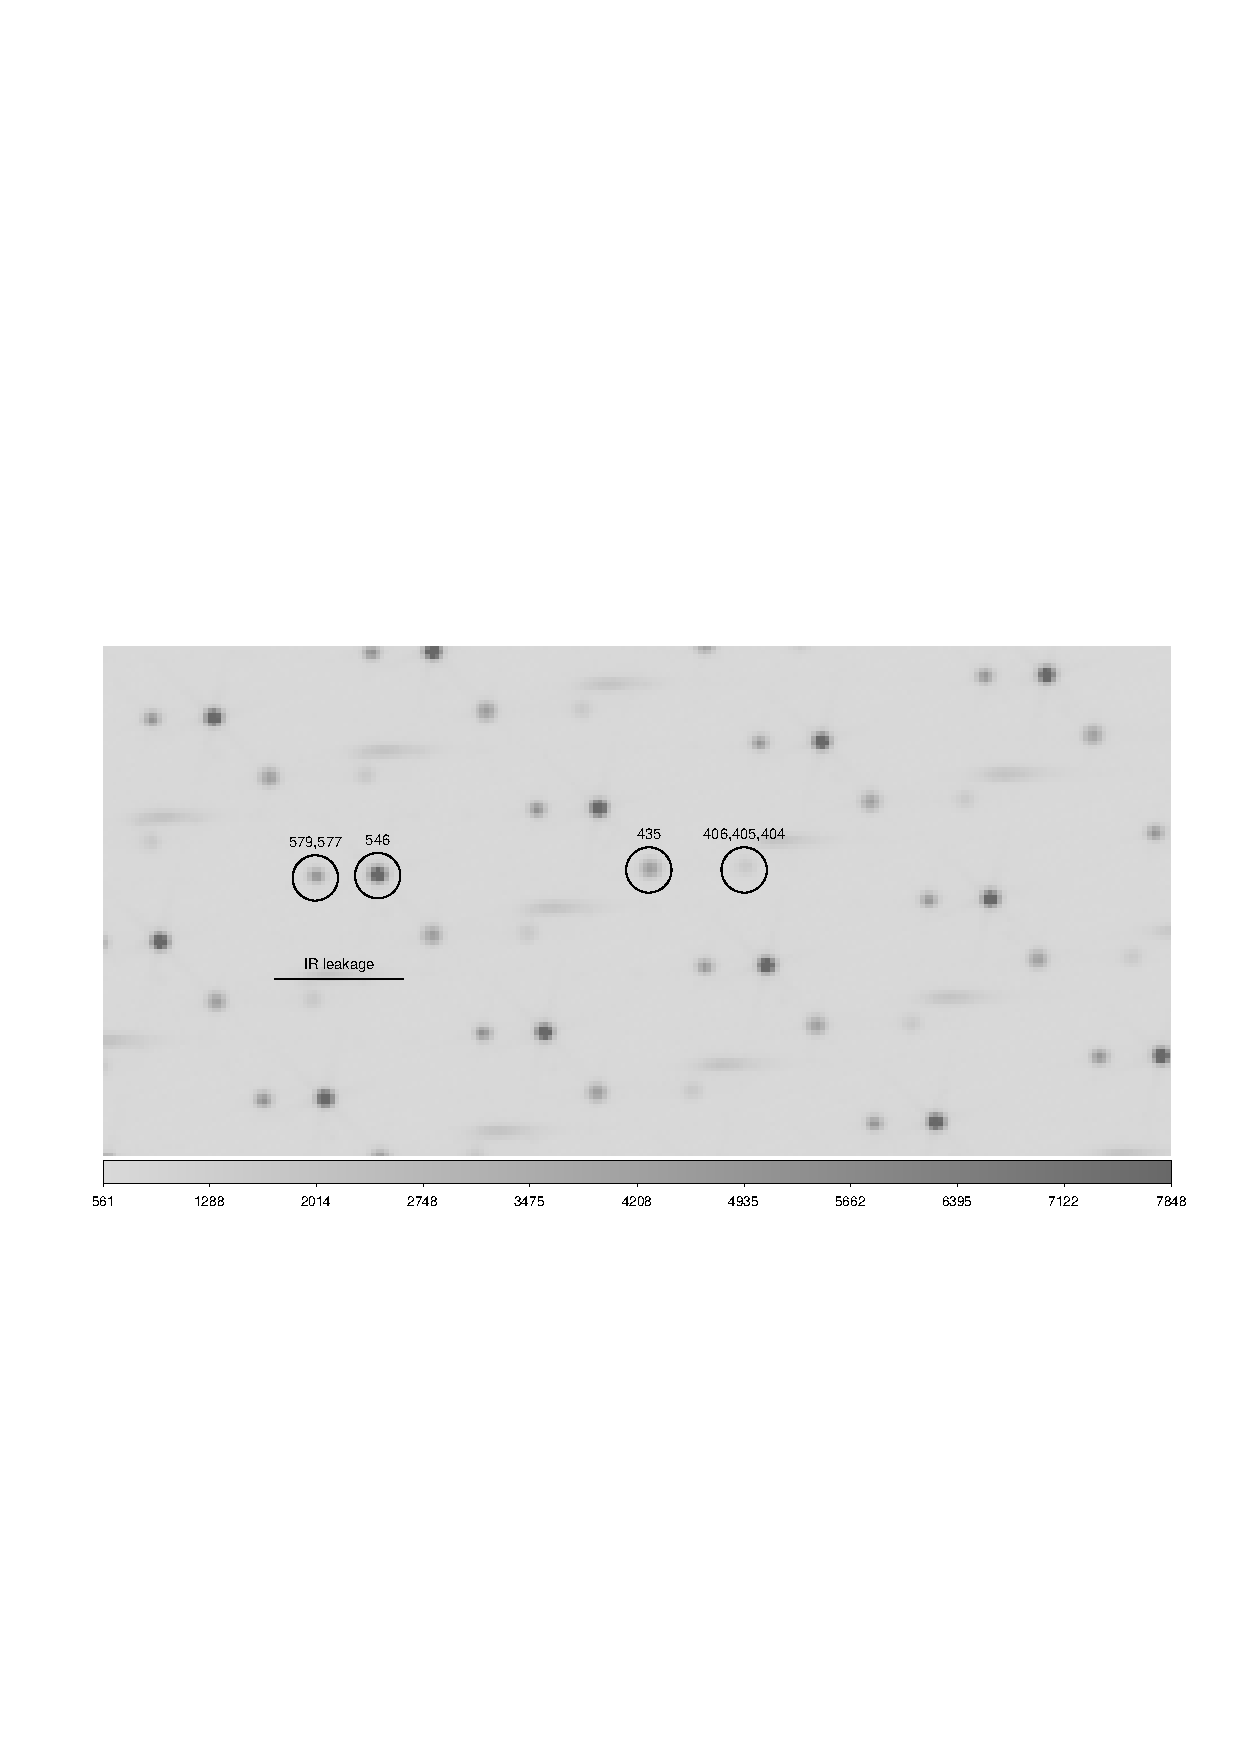
\includegraphics[width=3.0in]{figures/hg_2013_06_22_16_13_20.pdf} 
   \caption{Mercury arc lamp spectrum taken by illuminating the dome and exposing the spectrograph for two minutes. Key emission lines are identified with their wavelength in nanometers. Some lines are blended, and their components are listed. A broad broad line in the infrared portion of the spectrum appears, the source of this line is unidentified. The difference in pixel positions between the redder pair of lines is about 14 and for the bluer pair is 20. Based on the pixel distances and wavelength, it is clear that prism is achieving the designed constant resolution of $100\pm20$. }
   \label{fig:focal_plane}
\end{figure}

%435 @ 947
%405 @ 967
% DL = 30, Dp = 20
% 415/100 = 4.15
% 20 pix / pupil size * 4.15 = 35

%546 @ 887
%579 @ 873
% DL = 33, Dp = 14
% 560/100 = 5.6
% 14 pix / pupil size * 5.6 = 33

\subsection{Rainbow camera}

The  functional specifications of the rainbow-camera (RC) imager are as follows. The imager must sample the typical 1.2-arcsecond seeing of the Palomar 60-inch telescope and has a plate scale of $\sim0.4$ arcsecond per pixel. The purpose of the RC is to measure atmospheric absorption in the spectrograph, and thus the RC's wavelength range must cover from u' to i'. The field of view and throughput are designed such that with 60-s exposures a star with signal-to-noise greater than 100 is common.

The rainbow camera (RC) is an imager that provides focused images from u to i band. The RC is designed to accept the incoming $f/8.75$ telescope beam, and demagnifies the telescope image by $\sim1.8\times$ to produce an optically flat $f/4.9$ beam. Most of the elements of the RC are off-the-shelf and thus we had little control of the as-built optical prescription. The as-built RC delivers a $f/4.7$ beam such that the $13.5 \mu$ pixels subtend about 0.395 arc second each.

The RC was designed by SBA as follows. A set of four dielectric filters\footnote{all filters are from the Astrodon corporation.} is arranged in a 2x2 grid some 20-mm away from focus. The camera is composed of Ohara $i$-line, fused silica, and calcium fluoride optics. The fused silica field lens places a telescope pupil near a 90-mm triplet designed, fabricated, coated, and placed in a small aluminum barrel by Edmund Optics (EO64-838). A doublet and two singlets operate on either side of the triplet. These serve to control aberrations and flatten the field. The positive elements are off-the-shelf fused silica lenses, while the negative elements are fabricated by Harold Johnson Optical Laboratories in Gardena CA.

In the laboratory, when fed with a 0.5-arcsecond image the RC delivers sub-arcsecond images in all bands [SAGI, CAN WE QUANITIFY THIS]?. During our observing run from 19 to 23 June 2013 our best images were 1.4 arcsecond in the r and i bands and 1.6 arcsecond in the u and g bands. The Palomar Observatory seeing monitor\footnote{The seeing monitor is a small telescope that images Polaris with 30-second exposures. ????} reported seeing of 1.0 arcsecond. The source of this discrepancy in image quality between  on-sky measurements and those reported by the seeing monitor, but it  RC optics.

\subsection{Doublet lens bonding}

The spectrograph optical design has four contact doublets. In principle, the throughput of these doublets should be near perfect as the fresnel loses at the glass-grease-glass interfaces would amount to BLAH percent. However, due to a miscommunication with our supplier ISP optics, the CaF2 elements were coated on both sides rather than on the air-facing side. Thus, the throughput is predicted to take a hit in the blue. In the future, our lens-element drawings will have arrows to each surface calling out the surfaces to be coated. The smallest doublet use an optical grease from BLAH. The element is held together in a small lens barrel with a commercial retaining ring.

Three of these are bonded together using a room-temperature vulcanizing (RTV) epoxy Sylgard-184 of Dow Corning. Compared to a variety of doublet-bonding glues, epoxies, and RTVs Sylgard-184 transmits well in the blue above 370 nm where most UV-curing epoxies have poor transmission below 400 nm; and also has a rubbery consistency that absorbs any mechanical stresses caused by coefficient of thermal expansion mismatches. Camera doublet 1/2 is composed of calcium fluoride and fused silica which have a coefficient of thermal expansion difference of almost ${\rm 18\times10^{-6}/^\circ C}$. 

Historical data accumulated over several years at the Palomar 60-inch telescope found that the median temperature at the Palomar 60-inch prime mirror is $10^\circ C$ with 99\% of the temperature range falling between 0.4 and $19.5^\circ C$. To minimize accumulated differential stress the doublets were bonded in a room at $13^\circ C$. We would have preferred the room's temperature to be set to Palomar's median of $10 ^\circ C$; however, no such room was available to us.

A written procedure describing almost one-hundred steps for bonding the doublets was followed for each pair. The procedure was developed by practicing on dummy lenses of similar diameter from Edmund optics. All told, 9 practice runs were made to develop the procedure. The initial procedure and tooling was inadequate and required a complete redesign. Detailing the design, practice, and redesign of this procedure and its missteps is beyond the scope of this work. The authors benefited from the help of J. Crane at Carnegie Observatories and ?? at the National Observatories who shared their techniques for Sylgard-184 bonding. 

The optical design called for the thickness of the Sylgard-184 bond to be 125 $\mu$. Bond thickness was controlled by using Kapton-tape shims. The shims were measured with a dial indicator on a pink granite bench. Both substrates were cleaned minutes before application of Sylgard-184 with red ``first contact'' cleaning solution. Pipettes were used to control the amount of Sylgard delivered to the lens. The concave lens was placed face up to collect the correct volume of Sylgard-184, while a small dab of Sylgard-184 was placed in the center of the convex lens to facilitate bonding as described in \cite{bessell2011}. The element was left to cure over five days at 13$^\circ$ C as suggested in the Dow Corning application note.

The camera 1/2 doublet was bonded backwards with Sylgard-184. Based on Table 1 in \cite{Lee:2003uk}, we discovered that soaking the doublet in toluene caused the Sylgard bondline to expand by a factor of about 1.3. The expansion of the bond delaminated the two lenses without any damage.

\subsection{Lens potting}

Most of the SED Machine lenses were potted into aluminum cells which in turned were stacked as ``poker chips''. In this section we describe this process. The underlying philosophy of our approach was to rely on the manufacturing of the optics and their mounts and have no adjustments built in (except for focus). 

The optics are made of materials including fused silica, calcium fluoride, and a variety of Ohara i-line glasses. The coefficient of thermal mismatch between the optics and 6061T6 aluminum ranges from $3 - 23 \times10^{-6}/^\circ C$.  To athermalize  the applied  stresses due to temperature changes, we potted the optics using a RTV.

Initial calculations suggested that each lens should have skinny bond lines with thicknesses of order 0.050 mm. With three materials and tunable bond thickness, assuming a linear CTE these skinny bond lines would achieve a zero-stress lens mount. The sensitivity of the bond line is such that small manufacturing variations lead to glass stresses on order of 8 GPa, more than a factor of two higher than our requirement of 3.4 GPa.

Instead we adopted a thick bond line of 0.9 mm where the RTV, which is elastic, absorbs mechanical stresses. Our calculations show that such thick bondlines induce stresses on order of 2 GPa over the temperature range. All lenses were potted with a Momentive room-temperature vulcanizing (RTV) 60. The blue Momentive SS4155 primer was used to ensure good adherence between the lens and aluminum cell. 

Though the optical mounts were manufactured to not allow any mechanical adjustments, we confirmed that each optics was centered to within 25 micron with tilts on order of 1 arcminute. The centeration and tilt of each optic was measured before potting with a Coordinate-Measuring Machine (CMM) that Prof. Ian McLean at the University of California Infrared Laboratory allowed us to use. Thus, each lens was placed in the cell, centered using a tooling pin, and the final location of each lens was measured. Though there are no adjustments made to the lens cell, the CMM was essential. In several cases small pieces of black paint ended up between the cell and its interface lip. These pieces of paint induced 10 arcminute tilts  and would have degraded image quality. 

A picture of the first camera cell post potting is shown in Figure~\ref{fig:cam12}. The RTV was too thick to meter with our air pressure metering system and imperfections in the size of each bead can be seen. All beads are at least 5 mm in diameter as designed.

\begin{figure}[h] %  figure placement: here, top, bottom, or page
   \centering
   \includegraphics[width=2.5in]{figures/cam_12.jpg} 
   \caption{The first camera doublet potted in the lens cell. Three vertical pins are used to locate the doublet and ensure it is centered within 25 micrometer. Tooling holes allow red RTV-60 to be injected  at 12 locations around the perimeter of the lens. Both }
   \label{fig:cam12}
\end{figure}



\subsection{Laboratory testing}

A variety of lens-level optical tests were performed using standard techniques described in a wide range of literature. The ultimate test of any system is its end-to-end performance and thus here we concentrate on the performance of the full SED Machine system.

[IS THIS SECTION NNECESSARY]?



\section{Observations}

\appendix
\section{Optical Prescription}

\section{Timeline of critical events}

\section{Comparison against predictions}

\section{Budget}

\section{Acknowledgements}

Our collaborators in Taiwan who developed the data reduction pipeline, Prof. Wing Ip, Prof. Choong Ngeow, Dr. Andreas Ritter, and Mr. Alex Ruddy also provided some feedback to the team for hardware.

The PDR review team made a number of valuable suggestions.

Jack T.C. Davis, now at Spacex, served as the main mechanical designer.

Paul Gardener, the Palomar Chief Engineer, provided a wide range of mechanical design support.

Ernest Croner served as an electronics technician for the shutters and LED projection system.

Marin Anderson helped bond elements together.

Donal O'Sullivan

Pavan 

\begin{thebibliography}{}

\bibitem[Bacon et al.(1995)]{bacon95} Bacon, R., Adam, G., Baranne, A., et al.\ 1995, \aaps, 113, 347 

\bibitem[Bacon et al.(2001)]{bacon2001} Bacon, R., Copin, Y., Monnet, G., Miller, B. W., Allington-Smith, J. R., Bureau, M., et al. (2001). The SAURON project - I. The panoramic integral-field spectrograph. Monthly Notices of the Royal Astronomical Society, 326(1), 23�35. doi:10.1046/j.1365-8711.2001.04612.x

\bibitem[Bessell et al.(2011)]{bessell2011} Bessell, M., Bloxham, G., Schmidt, B., and Keller, S. 2011. SkyMapper Filter Set: Design and Fabrication of Large Scale Optical Filters. arXiv.org.

\bibitem[Sugai et al.(2010)]{sugai2010} Sugai, H., Hattori, T., Kawai, A., Ozaki, S., Hayashi, T., Ishigaki, T., et al. (2010). The Kyoto Tridimensional Spectrograph II on Subaru and the University of Hawaii 88�in Telescopes. Publications of the Astronomical Society of the Pacific, 122(887), 103�118. doi:10.1086/650397

\end{thebibliography}



\end{document}

